\section{Sleep Rhythm and Working Hours}

\subsection{Sleep Rythm}
To evaluate the significance of the punchcard in terms of sleep rhythm analysis, a small survey in a closed community has been made.
A selected group of ten people, who know each other well, has been selected for this purpose.
Furthermore, a subset of four people has been chosen which were going to be evaluated.
The data gathered for the test group only contained their leisure time contributions, as their work repositories were not open source.
All ten people then needed to assign the punchcard of those four persons to a specific person.
The specific task given to test group was to assign each punchcard to a specific person based on their knowledge about their sleep rhythm and leisure time behavior.

To this end, three quite similar patterns, where one contributor has a very regular sleep rhythm (Subfigure 2 in Figure~\ref{fig:punchcard-survey}) and one pattern of a practically inexistent sleep rhythm (Subfigure 1 in Figure~\ref{fig:punchcard-survey}) have been selected.

For the three similar graphs, no significant results could be assessed, as the assignments were more or less random.
The contributor with the irregular sleep rhythm, on the other hand, got correctly assigned in all cases.

Sadly, as such a survey needs very specific targeting and a long lead time for data collection, it could only be executed on a small set of subjects.
Anyhow the result of this survey indicates, that there exists a correlation between the structure of the punchcard and the sleep and leisure time commit behavior of a contributor, even if it can only be accurately assigned in extreme cases.


\begin{figure}[H]
    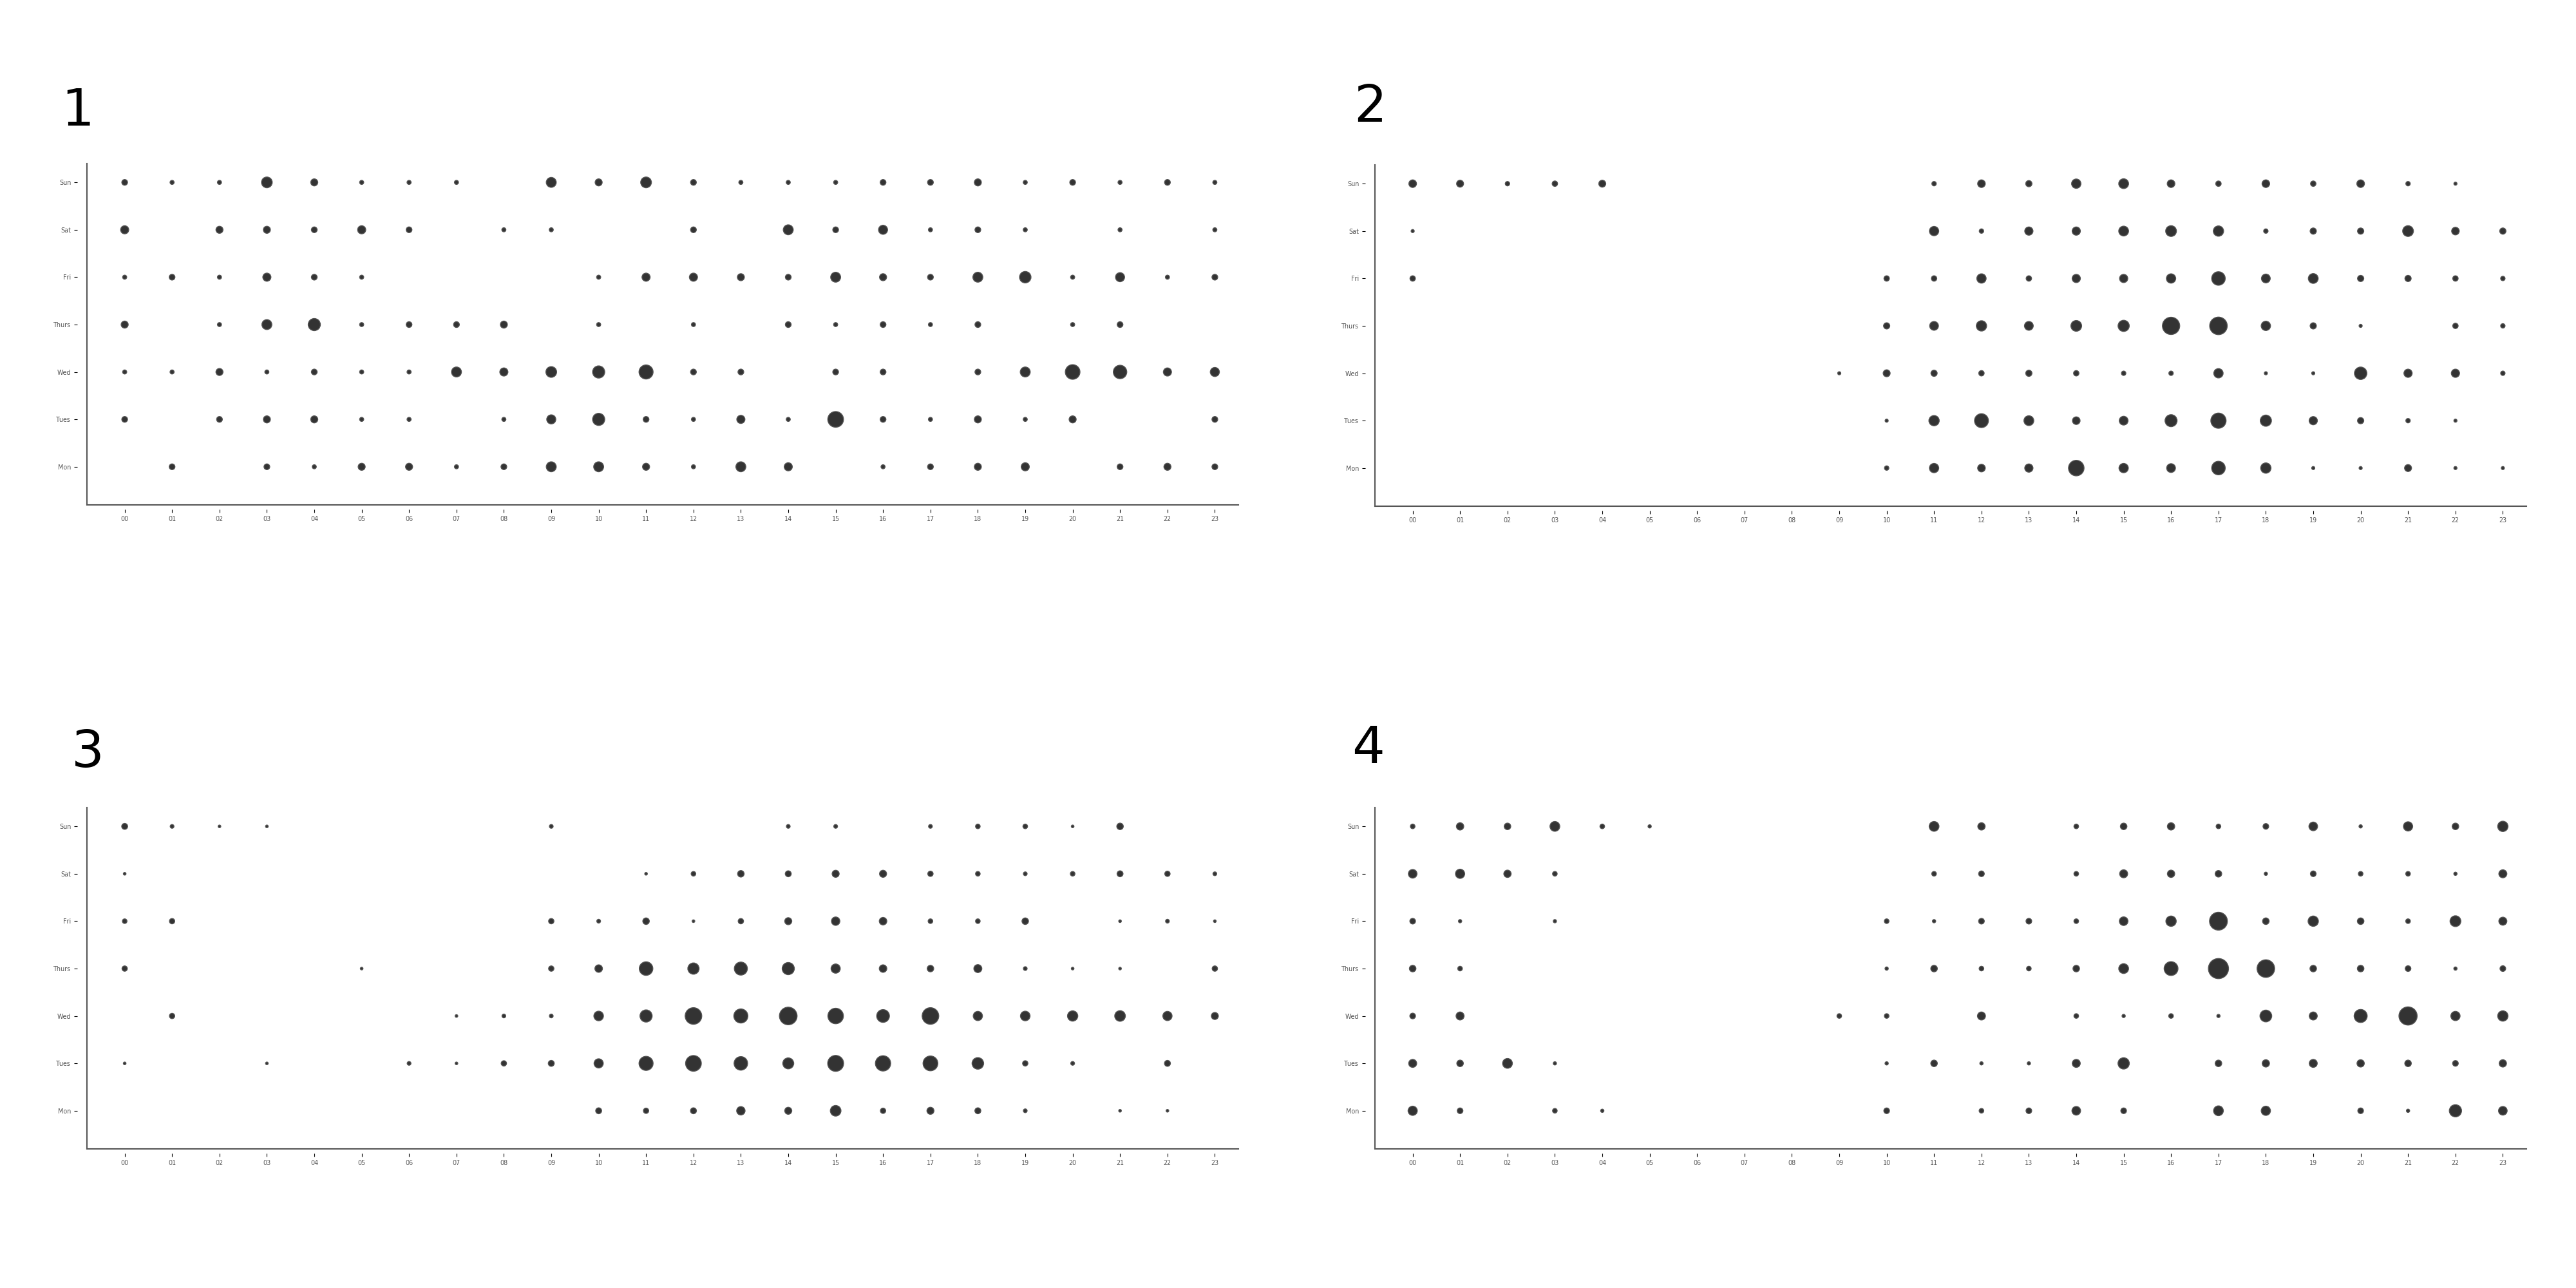
\includegraphics[scale=0.16]{./graphs/analysis/survey_combined}
    \centering
    \caption{The four punchcards used in the survey.}\label{fig:punchcard-survey}
\end{figure}

\subsection{Employee or Open-Source Contributor}
To determine whether a punchcard could be used to distinguish between an employee or an open-source volunteer, the results of the clustering described in Section~\ref{punchcard-implementation} has been utilized.
For this approach, two assumptions have been made.
A usual employee works between Monday and Friday during the day and only as an exception at the weekend, an example cluster can be seen in Figure~\ref{fig:normal-office-hours}.
An open-source volunteer works outside of the usual work shifts, which means early and late during weekdays and at the weekend, an example cluster can be seen in Figure~\ref{fig:leisure-time-hours}.

\begin{figure}[H]
    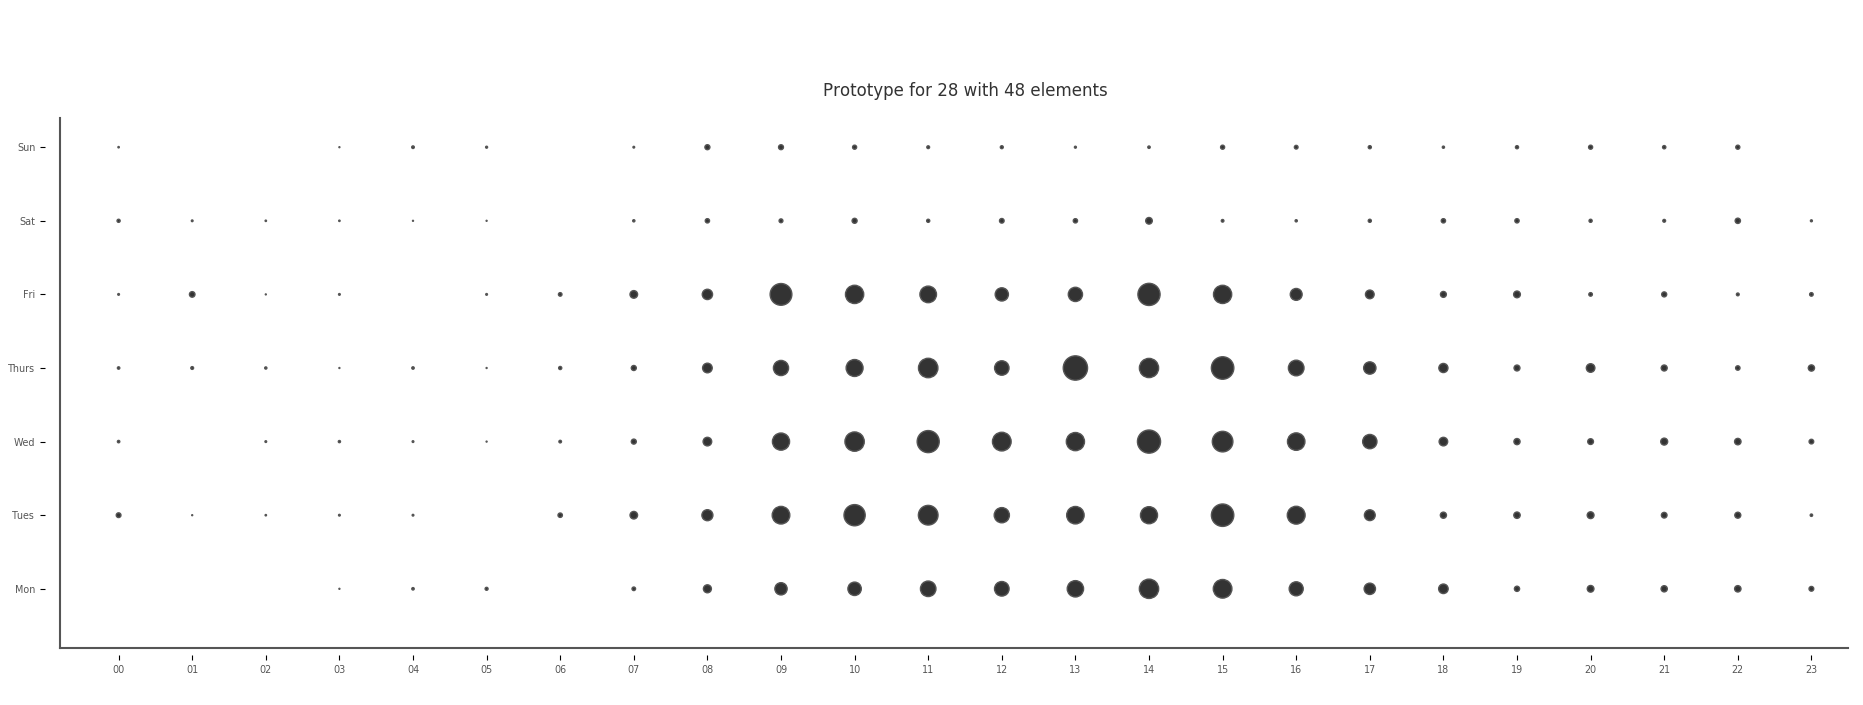
\includegraphics[scale=0.32]{./graphs/analysis-affinity/28}
    \centering
    \caption{Punchcard of an example from an affinity propagation cluster with normal work shifts.}\label{fig:normal-office-hours}
\end{figure}

For each assumption, two representative clusters have been chosen and ten random persons have been selected from each cluster.
The manual verification is conducted by checking if the contributor mainly contributes to repositories which belong to the registered employee.
If no employee is registered, but other sources such as a homepage are provided, the information of these sources is checked for possible employee details as well.
In case no employee exists, it is examined whether the contributor pushes to their own and to open-source projects or rather to the repositories of a specific company.

\begin{figure}[H]
    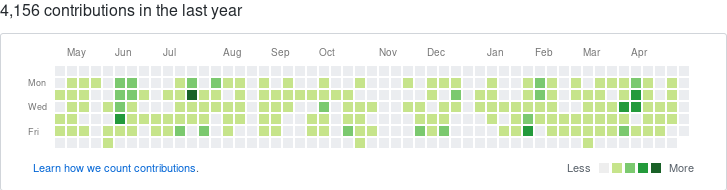
\includegraphics[scale=0.6]{./graphs/contribution-overview-alxhub}
    \centering
    \caption{Github contribution overview of a Google developer with the nickname alxhub.}\label{fig:github-contribution-overview}
\end{figure}

For this purpose, the Github contribution overview on the contributors' profile page has been used.
An example of such an overview can be seen in Figure~\ref{fig:github-contribution-overview}.
It provides a good overview of the usual weekday work pattern over the last year and allows to quickly inspect the repositories a contributor committed to at a specific month.

\begin{figure}[H]
    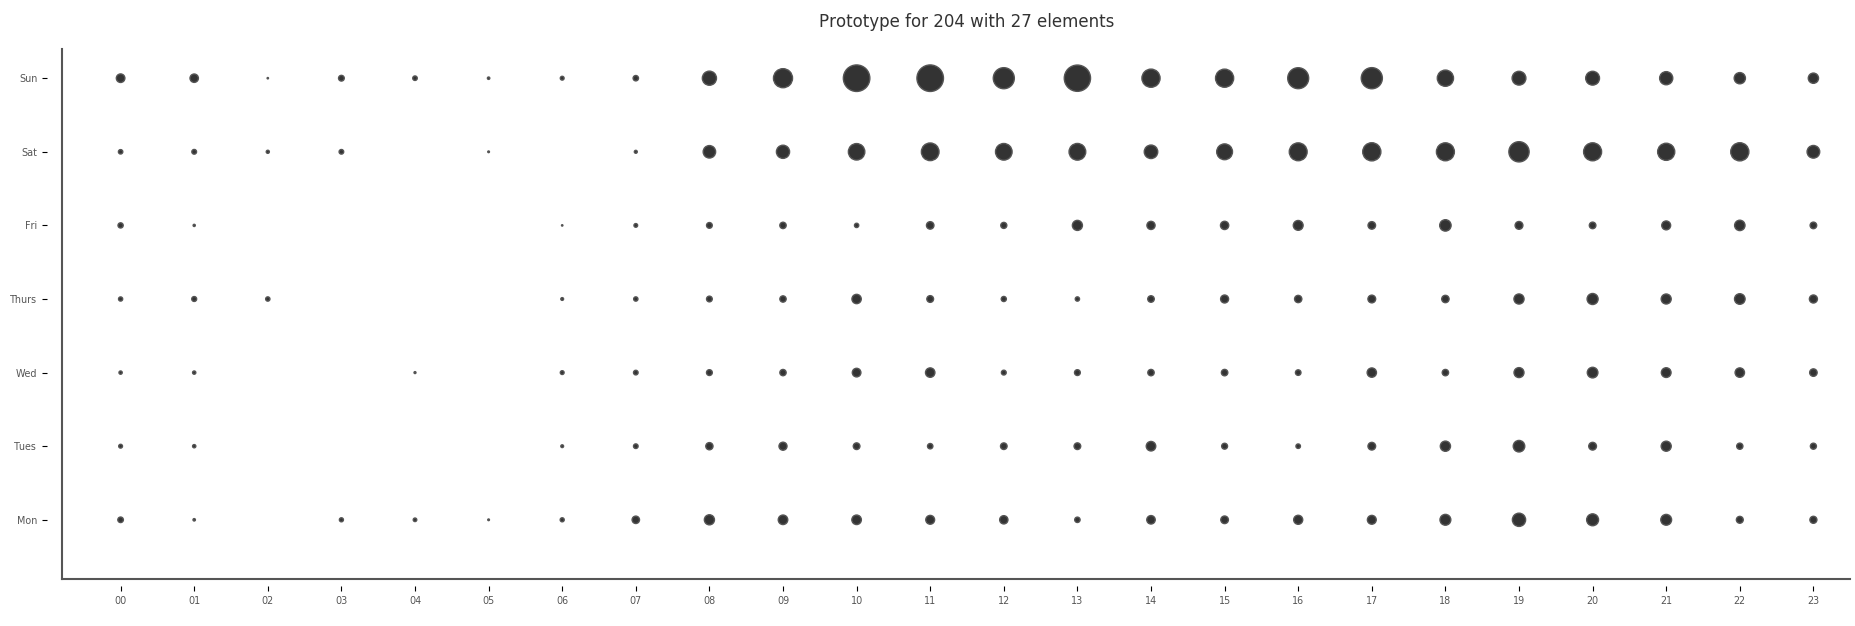
\includegraphics[scale=0.32]{./graphs/analysis-affinity/204}
    \centering
    \caption{Punchcard of an example from an affinity propagation cluster with a weekend tendency.}\label{fig:leisure-time-hours}
\end{figure}

The representatives for the usual five-day week commit behavior were surprisingly accurate.
19 out of 20 considered contributors were mainly working on projects of their companies, with occasional commits to other open source projects.
For the remaining contributor, it could not be determined if they work for a company.

\begin{table}
    \begin{center}
        \begin{tabular}{|c c c c c|}
            \toprule
            Nickname & Employer & Main projects & Work related & Overall commits more than 90\% to work related projects \\ [0.5ex]
            \midrule \midrule

            brettfo              &   Microsoft         &  visualfsharp                     &   yes             &    no \\
            \midrule
            aputinski            &   Salesforce        &  Salesforce                       &   yes             &    yes \\
            \midrule
            alxhub               &   Google            &  Angular                          &   yes             &    yes \\
            \midrule
            MatrixFrog           &   Google            &  Google Projects                  &   yes             &    yes \\
            \midrule
            ryanemerson          &   Red Hat           &  Infinispan                       &   yes             &    no \\
            \midrule
            garagatyi            &   Red Hat           &  Eclipse and related projects     &   yes             &    yes \\
            \midrule
            eternoendless        &   PrestaShop        &  PrestaShop                       &   yes             &    yes \\
            \midrule
            initvector           &   vanilla           &  vanilla                          &   yes             &    yes \\
            \midrule
            kyhavlov             &   HashiCorp         &  HashiCorp                        &   yes             &    no \\
            \midrule
            XenoPhex             &   CloudFoundry      &  CloudFoundry                     &   yes             &    yes \\
            \midrule
            gjoranv              &   unknown           &  vespa-engine/vespa               &   probably        &    yes \\
            \midrule
            doolse               &   Equella           &  Equella                          &   yes             &    yes \\
            \midrule
            leplatrem            &   Mozilla           &  Mozilla/Kinto                    &   yes             &    yes \\
            \midrule
            StrongMonkey         &   Rancher Labs      &  Rancher Labs                     &   yes             &    no \\
            \midrule
            lukaseder            &   jOOQ              &  jOOQ                             &   yes             &    yes \\
            \midrule
            DaazKu               &   vanilla           &  vanilla                          &   yes             &    yes \\
            \midrule
            brettcannon          &   Microsoft         &  Microsoft/Python                 &   yes             &    yes \\
            \midrule
            isidorn              &   Microsoft         &  Microsoft Projects               &   yes             &    yes \\
            \midrule
            jackhorton           &   Microsoft         &  Microsoft Projects               &   yes             &    yes \\
            \midrule
            glasserc             &   Mozilla           &  Mozilla/Kinto                    &   yes             &    yes \\
            \midrule
            nickwei84            &   CloudFoundry      &  CloudFoundry                     &   yes             &    yes

        \bottomrule
        \end{tabular}
        \captionof{table}{Employee cluster evaluation.}\label{tbl:employee-cluster-evaluation}
    \end{center}
\end{table}


The representatives for the leisure time commit behavior are mostly correct as well.
15 out of 20 considered contributors were irregularly contributing to either work unrelated open-source projects or to their own projects.
See Appendix~\ref{tbl:leasure-time-cluster-evaluation} for a table with the results of the leisure time cluster evaluation.
The remaining five contributors were either contributors working and committing to their employee's projects, but also to their own and open source projects or employees with an untypical commit behavior.

This analysis shows quite well, that there is a correlation between the assumed patterns and the Github commit behavior or the usage of their Github accounts.
Unfortunately, the evaluation process for these results is very time consuming and thereby only a relatively small sample (n=40) has been chosen.
As it is not trivial to link the employee of a contributor to all their funded projects, all verification needed to be conducted manually.


\subsection{Bot Detection}
Another possible attack, that opened up during the creation of the clusters, was the detection of automatically committing programs, so-called \emph{bots}.
Several clusters showed a very consistent commit behavior around a specific hour, such a punchcard can be seen in Figure~\ref{fig:bot-punchcard}.

\begin{figure}[H]
    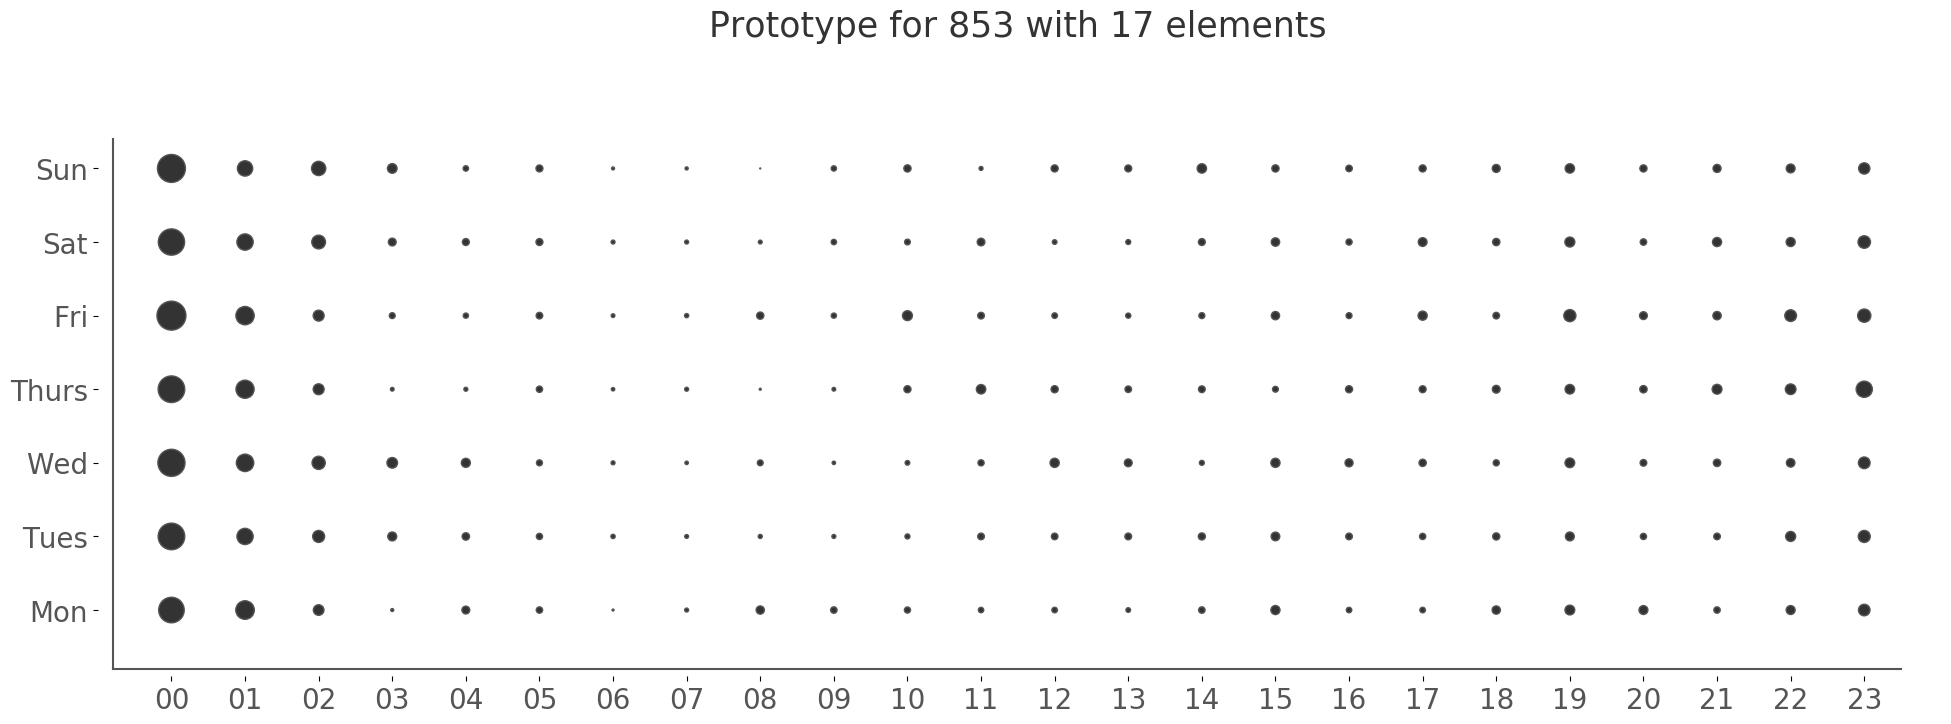
\includegraphics[scale=0.32]{./graphs/analysis/bot-punchcard}
    \centering
    \caption{Punchcard with an extraordinary commit pattern around midnight.}\label{fig:bot-punchcard}
\end{figure}

In the following, I implemented an algorithm, which simply detected centroids with an extremely equally distributed pattern or patterns with a spike at a specific hour.
After a manual revision of the clusters detected by this methodology, it became apparent that only a very small subset of those clusters actually contained bots.
And even if the cluster contained bots, there usually were only one or two of a much larger pool of cluster members.

Detection of bots in the outliers, which were not assigned to any cluster, did not seem to be promising as well.
Manual revision of over 100 possible candidates led to not a single bot.
After reviewing these results, I decided that there is currently no viable approach to this problem.


\subsection{Fingerprinting}
Another possible attack was to fingerprint a contributor and create a unique identifier by analyzing their commit behavior.

This attack soon proved to be unfeasible, as the pattern of a contributor significantly differs from month to month, as can be seen in Figure~\ref{fig:october-punchcard} and Figure~\ref{fig:november-punchcard}.

\begin{figure}[H]
    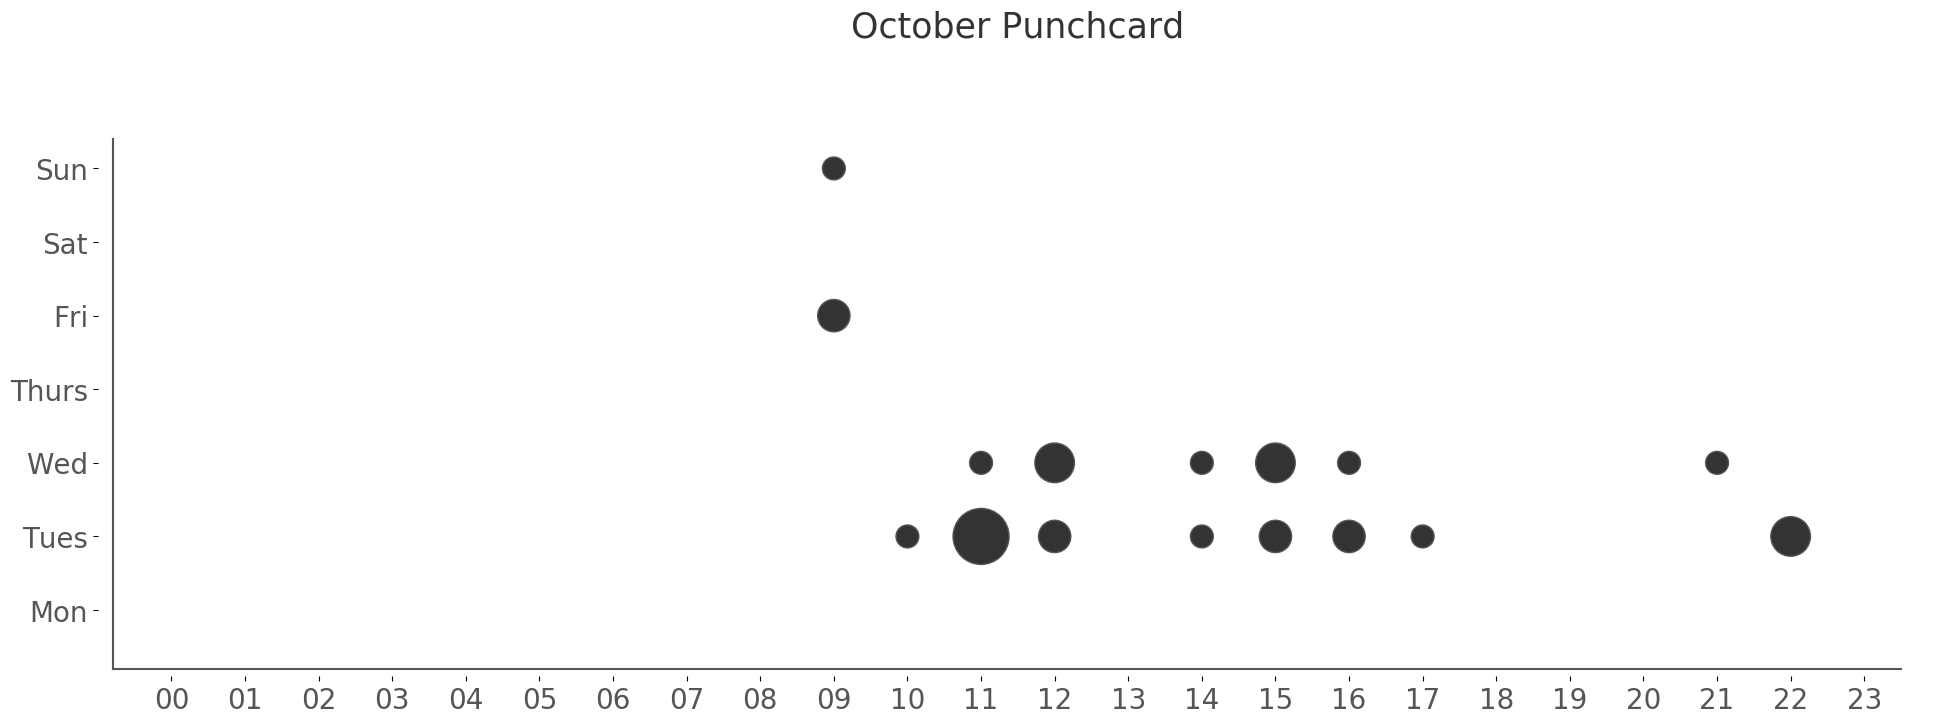
\includegraphics[scale=0.32]{./graphs/analysis/october-punchcard}
    \centering
    \caption{Punchcard of the author from October 2017.}\label{fig:october-punchcard}
\end{figure}

\begin{figure}[H]
    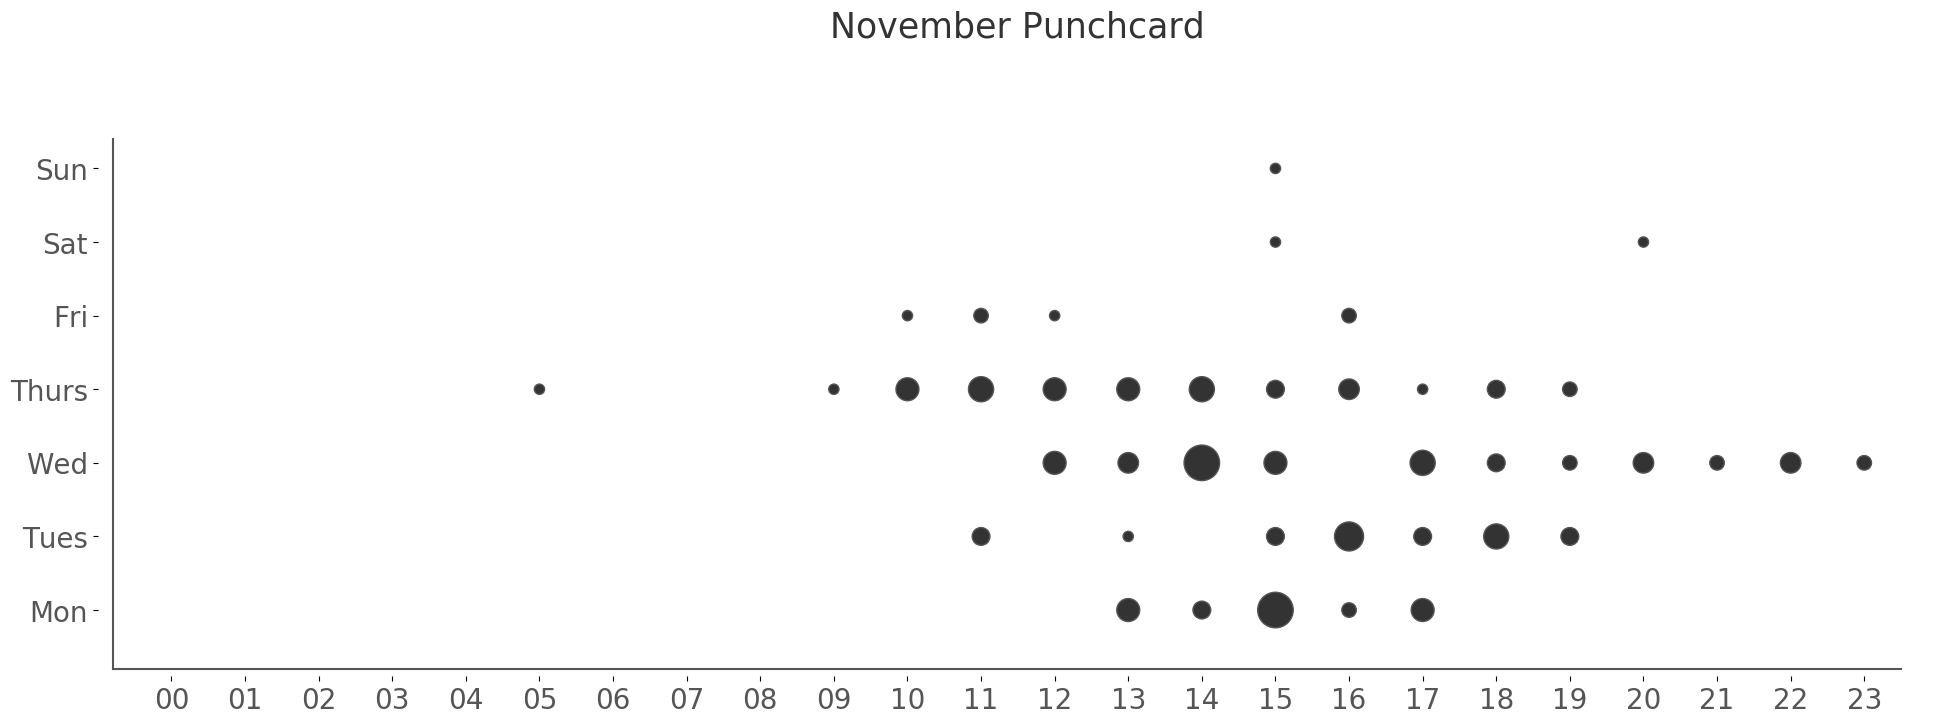
\includegraphics[scale=0.32]{./graphs/analysis/november-punchcard}
    \centering
    \caption{Punchcard of the author from November 2017.}\label{fig:november-punchcard}
\end{figure}

If the interval of a year is considered and the compared interval is shifted by a single month, the occurring changes are not that drastic, but still too different to see a consistent pattern over a longer time.
The commit behavior of people seems to be too inconsistent to create a unique fingerprint.
